\chapter{Event and Population Analysis}\label{ch:analysis}

    Using the population models described in Chapter \ref{ch:synthesis}, one can derive
    the properties of NSBH mergers as seen in the GW as well as EM regimes.
    Specifically, an important aspect of NSBH mergers is what fraction of mergers
    actually produce a prompt component which will be detectable by present-day
    Gamma-ray detectors, such as INTEGRAL. A related aspect is the dependence of this
    fraction on the priors which go into creating these populations. Specifically,
    different black hole spin prior distributions should affect the number of detectable
    prompt emissions, and so this behaviour is worth investigating.  Furthermore, this
    population synthesis framework also helps to investigate the rate density of NSBH
    mergers which lead to observalble SGRBs, which can then be compared to the rate
    derived currently from purely EM observations.\\
    Additionally, events seen solely in the GW regime without any confident EM
    counterparts may be analysed using the framework set up here. Using the posterior
    distributions for the component masses, spins etc., derived from GW strain data
    analysis, one can derive the corresponding remnant, dynamic and disc masses from
    which the jet energetics can be derived. Under the assumptions of the underlying
    model, this process of computation can then help eliminate or give credence to the
    existence of EM counterparts for certain GW-only events.

\section{Analysis of Population Synthesis Models}

    From the description of the population models given in Chapter \ref{ch:synthesis},
    it is clear that there are three classes of populations, classified by the black
    hole spin population that is used. Specifically, the three classes of populations
    are:

    \begin{itemize}

        \item \textbf{Class I} -- this uses the standard \textsc{truncated} BH mass
            distribution with a contant NS mass of 1.4 M$_\odot$. The BH spin
            distribution is the beta distribution from \cite{abbott_2020B}, and the NS
            spin is set identically to 0 for all samples (see \ref{sec:ns_pop}
            for reasons on why this assumption is valid). The remaining NS parameters
            and their computation (such as the NS compactness, tidal deformability etc.)
            are described in \ref{sec:ns_pop}, and thus is omitted here for brevity.

        \item \textbf{Class II} -- here, the BH spin distribution is assumed to be
            uniform between [0, 1). The rest of the binary parameter distributions are
            the same as in Class I.

        \item \textbf{Class III} -- here, the BH spin is a "restricted" Gaussian
            distribution between [0, 1), and 0 elsewhere. More rigorously, the
            distribution is defined as follows:

            \begin{equation}
                \mathcal{P}(\chi_{BH}) =
                    \begin{cases}
                        K \exp \left[
                                - \left(
                                    \dfrac{\chi_{BH}-\mu}{\sigma}
                                  \right)^2
                            \right], &\text{ if } \chi_{BH} \in [0, 1) \\
                        0, &\text{ otherwise }
                    \end{cases}
            \end{equation}

            where K is a normalization constant, $\mu$ and $\sigma$ are the mean and
            standard deviation of the distribution.  For the purposes of being general,
            samples are drawn from distributions with $\sigma = 0.2$ and $\mu = 0.2,
            0.5, 0.7$.  The rest of the binary parameter distributions are the same as
            in classes I and II.

    \end{itemize}

    For each population, 10$^5$ samples are drawn from the relevant populations. Using
    the samples, the various mass parameters required to compute the energetics of the
    jet are calculated using Eqs. \ref{eq:m_out}--\ref{eq:constraint}. Then, using Eq.
    \ref{eq:e_kin_jet}--\ref{eq:eiso}, the jet structure is imposed and for each event
    the value of $E_{iso}(\theta_v)$ is computed. These are then converted into fluences
    using the equation:

    \begin{equation}
        \mathcal{F} = \dfrac{E_{iso}(\theta_v)}{4\pi d_L^2}
    \end{equation}

    This is done in order to ascertain the detectability of the prompt emission, with a
    typical gamma-ray detector, such as the INTEGRAL satellite, as a reference. The
    INTEGRAL satellite has a lower fluence cutoff of $2 \times 10^{-7}$ erg, and so with
    respect to this detector, any event with a fluence lower than this value will be
    considered a non-detection. Albeit this is a tight restriction, it helps to
    ascertain the rough number of detections versus non-detections.\\
    Similarly, with the binary parameters set by the sampling process, the GW network
    SNR is computed with the RWF as the GW template, using
    Eqs.\ref{eq:rho}--\ref{eq:freq_integral}. The detector network configuration
    consisting of Advanced LIGO (LIGO-Livingston, L1 and LIGO-Hanford, H1) and
    VIRGO (V1) detectors was set up using PyCBC's \texttt{detector} module, which builds
    up the detector locations, orientations, location phase factors etc. For all three
    detectors, the Advanced LIGO Design sensitivity was used as an approximation for
    their respective future configurations. This was done, since with the current
    network configuration, there have been no confident detections of NSBH mergers which
    have \textit{also} had an EM counterpart.\\
    The results of the simulations are given below, with each population producing a
    particular number of NSBH binary merger events seen in:

    \begin{enumerate}

        \item The GW regime alone: these are events whose GW network SNR is calculated
            to be higher than the network SNR threshold of 10.

        \item The EM regime alone: these are events whose simulated gamma-ray fluence
            is calculated to be above the INTEGRAL fluence limit of $2 \times 10^{-7}$
            erg.

        \item The GW \textit{and} EM regimes both: these are events which satisfy both
            the GW and EM `cutoffs', and thus represent joint detections.

    \end{enumerate}

    These numbers are collected together in Table \ref{tab:popln_numbers} for each
    population class. From this table it is evident that the spin distribution heavily
    affects the number of EM-only events, and by extension the number of joint events.\\
    This can be explained by looking at the dependence of $M_{\mathrm{disc}}$ on the BH
    spin, from Eq.\ref{eq:disc_mass}, for a fixed mass ratio. Since a highly spinning
    black hole produces more tidally disrupted material for a given mass ratio than a
    low spinning black hole, binaries with a higher black hole spin are more likely to
    produce a more massive disc, assuming not much mass is lost as dynamical mass.
    This dependence of $M_{\mathrm{disc}}$ is shown below in Fig. \ref{fig:m_disc}.

    \begin{table}[H]
        \centering
        \caption{Fix this table!}
        \begin{tabular}{cccc}
            \toprule

                &
            \begin{tabular}[c]{@{}c@{}}
                Events detected \\ via GW only
            \end{tabular} &
            \begin{tabular}[c]{@{}c@{}}
                Events detected \\ via EM only
            \end{tabular} &
            \begin{tabular}[c]{@{}c@{}}
                Events detected \\ via GW + EM
            \end{tabular} \\

            Class I & 26 & $\sim$12000 & 0 \\

            Class II & 832 & $\sim$12000 & 300 \\

            Class III ($\mu = 0.2$) &
            19 & $\sim$12000 & 0 \\
            Class III ($\mu = 0.5$) &
            266 & $\sim$12000 & ? \\
            Class III \\ ($\mu = 0.7$) &
            882 & $\sim$12000 & ? \\
            \bottomrule
        \end{tabular}
        \label{tab:popln_numbers}
    \end{table}


    \begin{figure}[H]
        \centering
        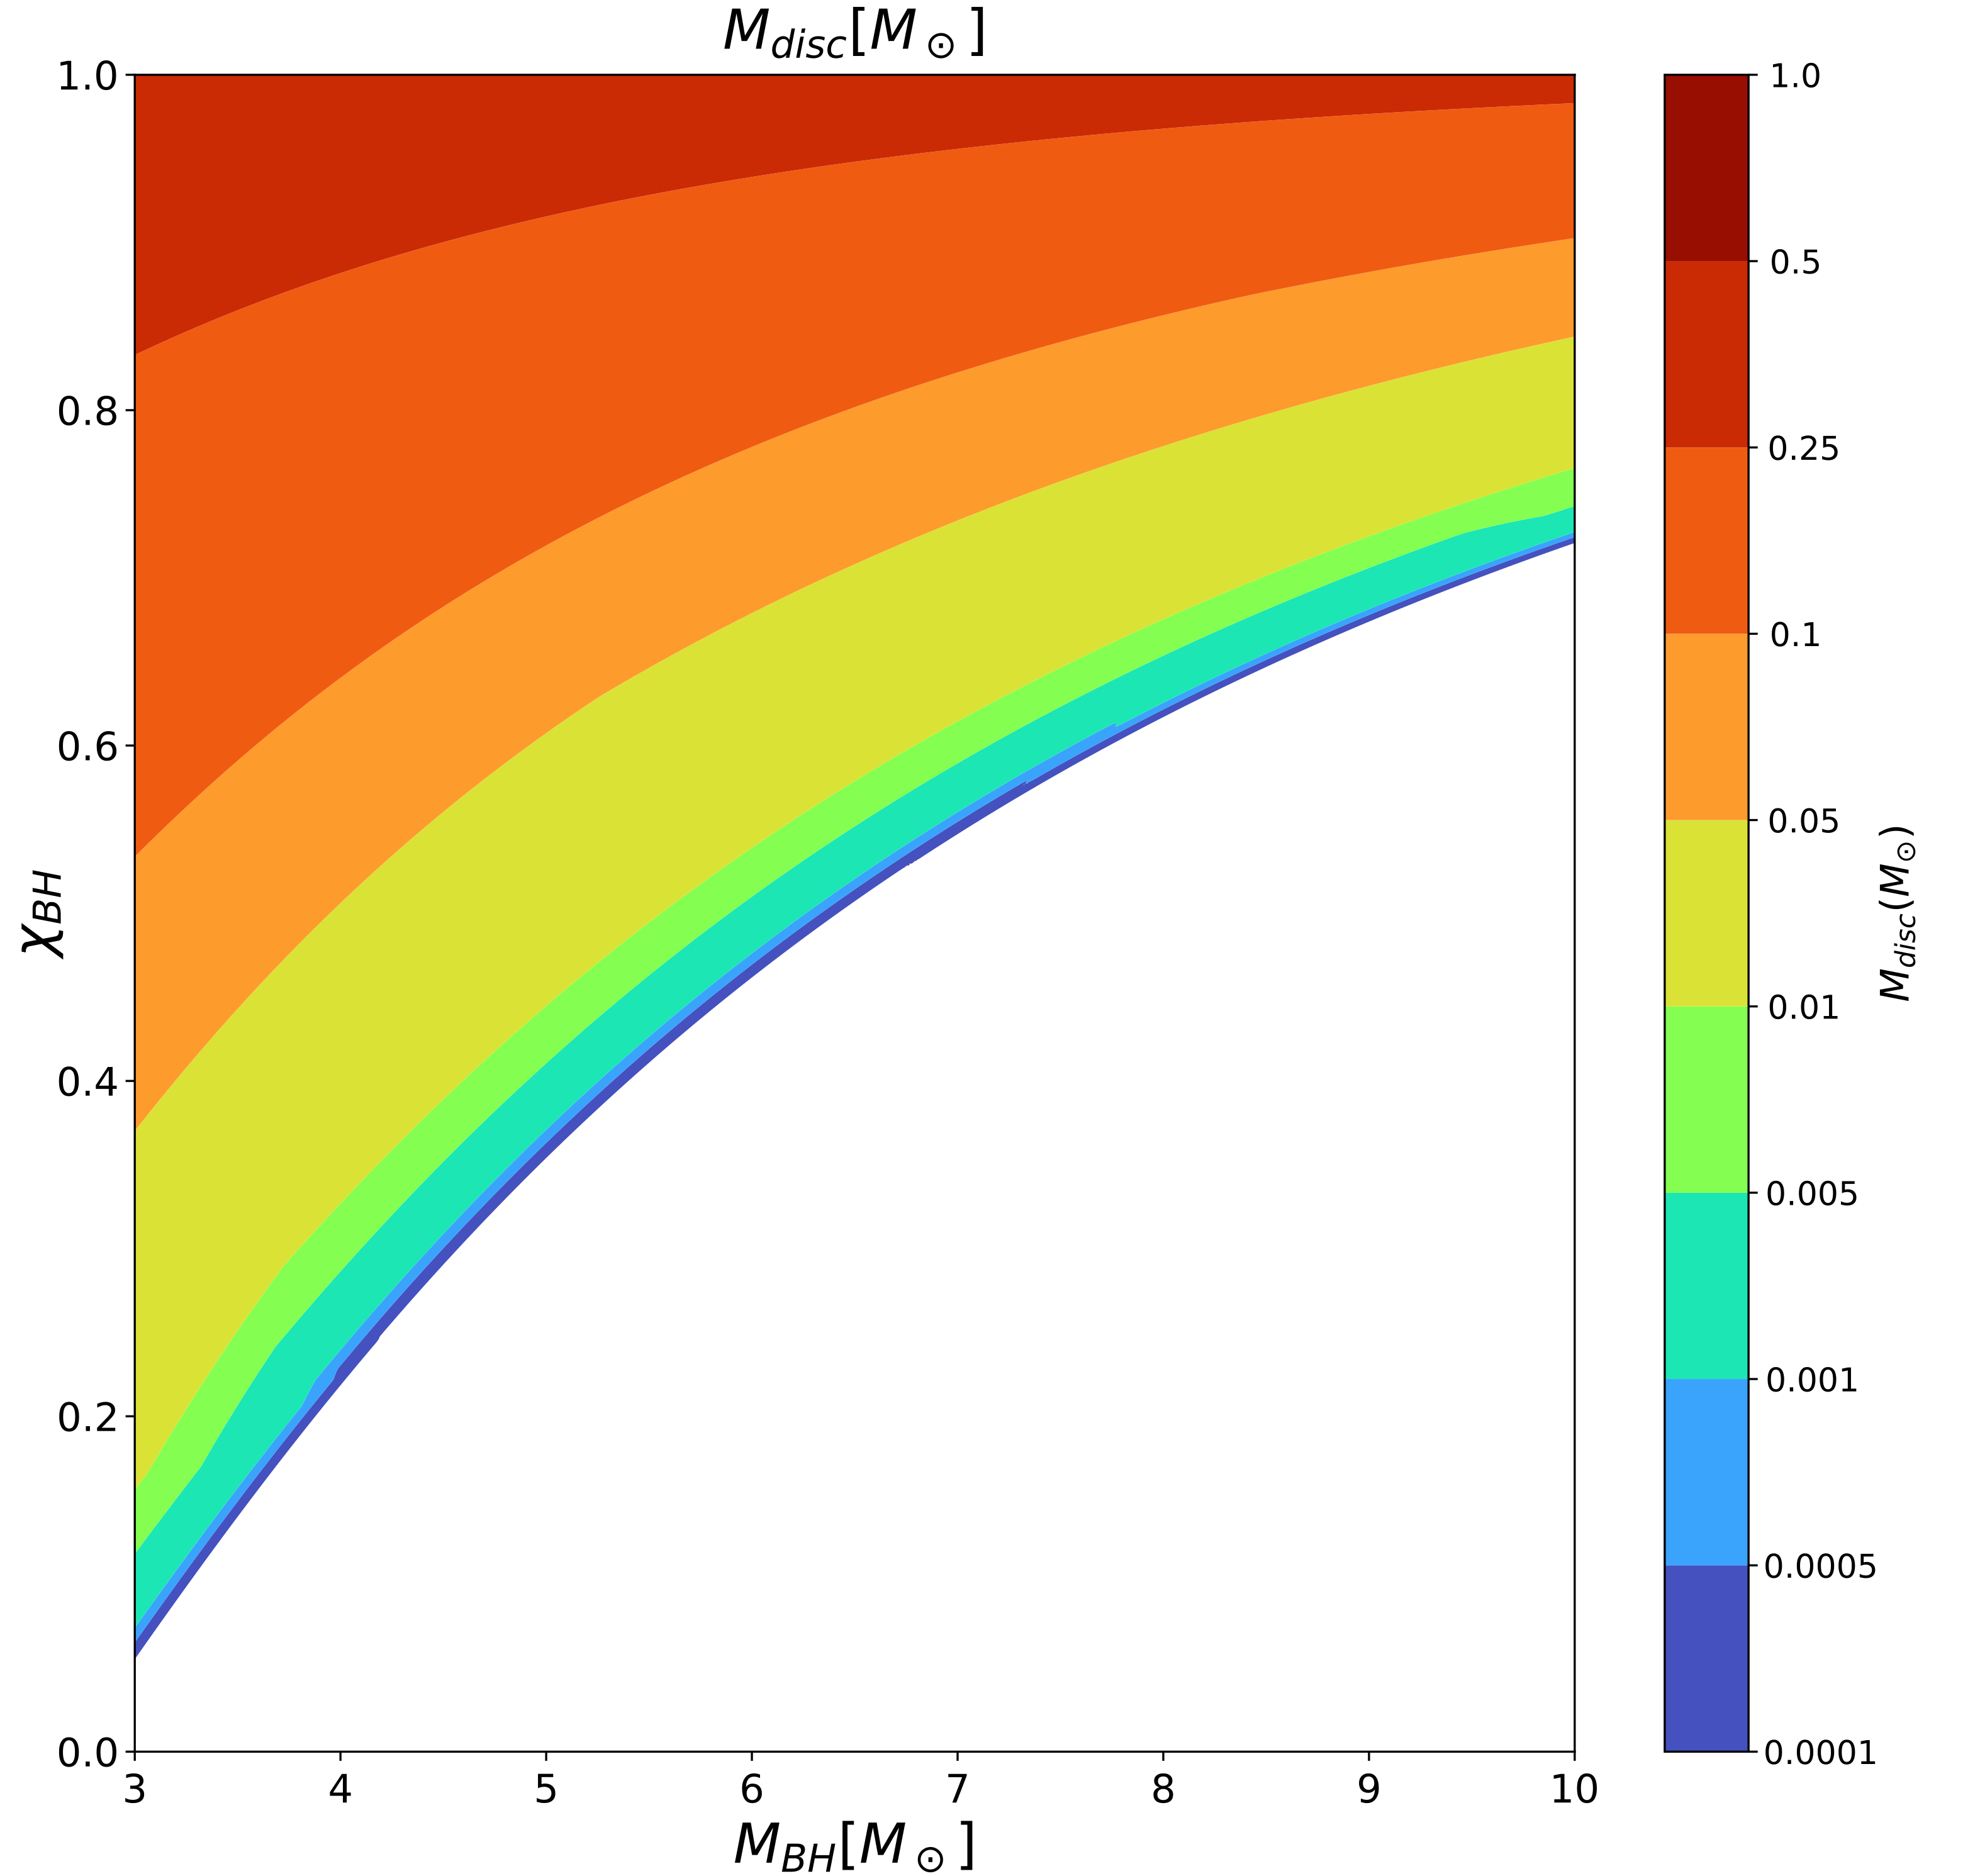
\includegraphics[width=0.8\linewidth]{m_disc}
        \caption[Variation of $M_{\mathrm{disc}}$ with $\chi_{BH}$ and $\mathcal{Q}$]{
            Variation of the disc mass with the mass ratio, $\mathcal{Q}$ and the black
            hole spin, $\chi_{BH}$. Note that the higher disc mass values are achieved
            when $\chi_{BH}$ is high and $\mathcal{Q}$ is low. Reproduced from
            \cite{barbieri_2019}.
        }
        \label{fig:m_disc}
    \end{figure}

    This then means that because populations with `high spin' distributions (such as the
    Class I population, or the Class III population with a high mean value for the spin
    distribution) have a higher proportion of high spin binaries, they have a higher
    number of EM and joint detections, since a more massive disc produces a more
    energetic jet from Eq.\ref{eq:eiso}, and thus increases the possibility of
    detections.

\section{Event Analysis}\label{sec:event_analysis}

    \subsection{GW190426}

        This event, as described in GWTC-2, has an astronomical source probability of
        42\% and a terrestrial event possibility of ~52\%. Even though this is the case,
        there is still speculation on whether this event could be an NS merger event.
        This is still possible since the priors used for the classification mechanism
        depend sensitively on  knowledge about the stocastic GW background and may
        change in the future, as more analysis is done on the GW noise observed as the
        LIGO/VIRGO interferometers operate.\\
        With this uncertainty in mind, asking the question of whether GW190426 could be
        an NSBH event is pertinent, and the current framework makes for a suitable test
        bed to test this hypothesis with.  Using the posterior samples released for the
        binary parameters associated with GW190426, which gives samples from the
        distributions for $M_{BH}, M_{NS}$ etc.  derived via the Bayesian parameter
        estimation process carried out by the LSC, the disc mass was computed for each
        set of binary parameters. Computing the disc mass is expeditious since it
        directly gives an estimate of how many sets of samples will be able to
        \textit{atleast launch} a jet, since if $M_{\mathrm{disc}} = 0$ for a particular
        set of samples, there is no possibility of detecting a jet from this particular
        binary.\\
        Fig. \ref{fig:mdisc_q_190426} is a representation of this analysis in the
        $\chi_{BH}-\mathcal{Q}$ plane. From that figure, it is seen that a very small
        fraction of posterior samples actually fall within the section of the parameter
        space where $M_{\mathrm{disc}} \neq 0$. This means correspondingly that the
        probability of the NSBH event GW190426 launching a SGRB jet at all is very low.
        This can be interpreted trivially to conclude that the event was of terrestrial
        origin, and thus it follows that it would not be compatible with the launching
        of an astrophysical jet. But non-trivially, one can also conclude that one of
        the following is true:

        \begin{itemize}

            \item The event GW190426 was a BNS binary merger event, which had a jet that
                was launched via other mechanisms.

            \item The event GW190426 was an NSBH binary merger event, but the jet was
                launched via a mechanism that is yet unknown. This means that the
                current analysis is invalid, and the true nature of jet launching is
                unknown.

        \end{itemize}

        The actual non-detection of such a jet could be either due to the inefficiency
        of the internal engine of such alternative mechanisms which powers the jet, or
        due to a large viewing angle, large enough that the jet was relativistically
        deboosted to below the thresholds of current-day gamma-ray observatories.


        \begin{figure}[H]
            \centering
            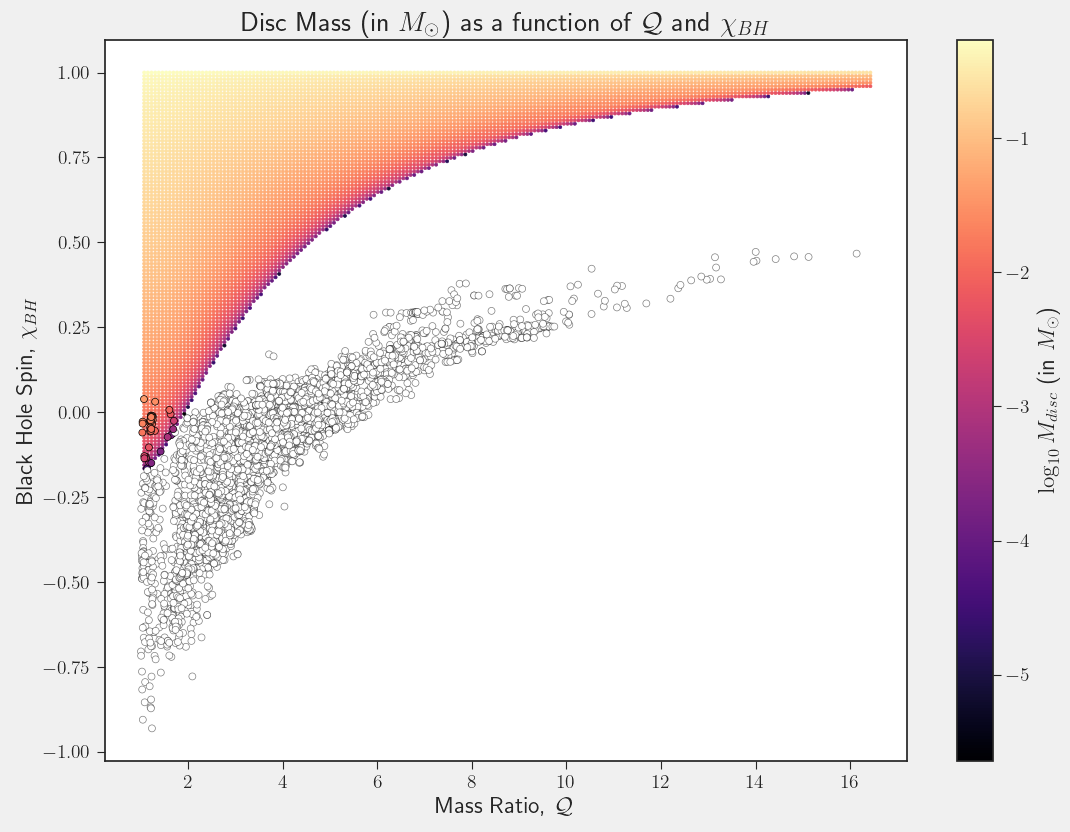
\includegraphics[width=0.9\linewidth]{mdisc_q_190426}
            \caption[GW190426 in the $\chi_{BH}-\mathcal{Q}$ plane]{
                GW190426 in the $\chi_{BH}-\mathcal{Q}$ plane. The color coding at a
                point in the plane indicates the value of $M_{\mathrm{disc}}$
                corresponding to that particular $\chi_{BH}$ and $\mathcal{Q}$.
                Unfilled black circles correspond to samples from the posterior
                distributions for GW190426, which have $M_{\mathrm{disc}} = 0$, and so
                cannot support jet launching, and filled black circles are those with
                $M_{\mathrm{disc}} \neq 0$.
            }
            \label{fig:mdisc_q_190426}
        \end{figure}



\section{Summary}
